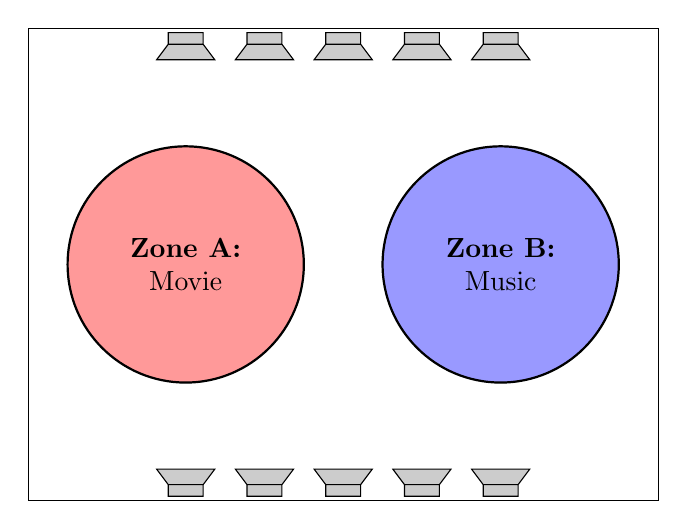
\begin{tikzpicture}
    \tikzset{
      Speaker/.pic={
        \filldraw[fill=gray!40,pic actions] 
        (-15pt,0) -- 
          coordinate[midway] (-front) 
        (15pt,0) -- 
        ++([shift={(-6pt,8pt)}]0pt,0pt) coordinate (aux1) -- 
        ++(-18pt,0) coordinate (aux2) 
        -- cycle 
        (aux1) -- ++(0,6pt) -- coordinate[midway] (-back) ++(-18pt,0) -- (aux2);
      }
    }

    \draw [draw=black] (0,0) rectangle (8,6);

    % Speakers on the top wall
    \pic[scale=0.7] at (2, 5.6) {Speaker};
    \pic[scale=0.7] at (3, 5.6) {Speaker};
    \pic[scale=0.7] at (4, 5.6) {Speaker};
    \pic[scale=0.7] at (5, 5.6) {Speaker};
    \pic[scale=0.7] at (6, 5.6) {Speaker};

    % Speakers on the bottom wall
    \pic[rotate=180, scale=0.7] at (2, 0.4) {Speaker};
    \pic[rotate=180, scale=0.7] at (3, 0.4) {Speaker};
    \pic[rotate=180, scale=0.7] at (4, 0.4) {Speaker};
    \pic[rotate=180, scale=0.7] at (5, 0.4) {Speaker};
    \pic[rotate=180, scale=0.7] at (6, 0.4) {Speaker};

    \draw[opacity=0.4, fill=blue] (6,3) circle[radius=1.5];
    \draw[thick] (6,3) circle (1.5) node[align=center] {\textbf{Zone B:}\\Music};
    \draw[opacity=0.4, fill=red]  (2,3) circle[radius=1.5];
    \draw[thick] (2,3) circle (1.5) node[align=center] {\textbf{Zone A:}\\Movie};
\end{tikzpicture}
